%! Author = francobregoli
%! Date = 12/03/2024

% Preamble
\documentclass[11pt]{article}

% Packages
\usepackage{amsmath}
\usepackage{graphicx}
\usepackage{float}
\usepackage{tikz}

% Document
\begin{document}

    \section{Jerarquía de Chomsky de lenguajes}

    La Jerarquía de Chomsky es una clasificación de lenguajes formales propuesta por Noam Chomsky en 1956. Se divide en cuatro niveles:

    \begin{enumerate}
        \item \textbf{Tipo 0:} Lenguajes recursivamente enumerables. Son generados por gramáticas de producción no restringida.
        \item \textbf{Tipo 1:} Lenguajes sensibles al contexto. Son generados por gramáticas de producción sensible al contexto.
        \item \textbf{Tipo 2:} Lenguajes independientes del contexto. Son generados por gramáticas de producción independiente del contexto.
        \item \textbf{Tipo 3:} Lenguajes regulares. Son generados por gramáticas de producción regular.
    \end{enumerate}

    Cada nivel de la jerarquía incluye a los niveles que le siguen, es decir, los lenguajes de tipo 1 incluyen a los de tipo 2 y 3, los de tipo 2 incluyen a los de tipo 3, y así sucesivamente.

    \bigskip % Agrega un salto de línea


    \section{Alfabetos}

    Un alfabeto es un conjunto finito de símbolos. Algunos ejemplos de alfabetos son:

    \begin{itemize}
        \item ASCII: Un estándar de codificación de caracteres basado en el alfabeto latino. Se utiliza principalmente en las computadoras y equipos relacionados.
        \item Unicode: Un estándar de codificación de caracteres que tiene como objetivo incluir todos los caracteres escritos posibles.
        \item \{0,1\} (alfabeto binario): Este es el alfabeto más simple y se utiliza en la computación digital y en la teoría de la información.
        \item \{a,b,c\}: Este es un ejemplo de un alfabeto simple basado en letras.
    \end{itemize}

    Cada alfabeto tiene su propio conjunto de reglas y convenciones que determinan cómo se utilizan los símbolos para formar secuencias más largas, como palabras o números.

    \bigskip % Agrega un salto de línea


    \section{Cadenas}

    Informalmente, si un alfabeto es el conjunto de listas, $\ast$ denota el conjunto de strings posibles usando los caracteres de $\Sigma$. $\epsilon$ denota el string vacío (string de longitud 0).

    Por ejemplo, $\{0,1\}^{\ast}$ = $\{\epsilon, 0, 1, 00, 01, 10, 11, 000, 001, . . . \}$

    Formalmente, una cadena (vamos a usar letras griegas para las cadenas) de longitud $n$ es una tupla de $n$ elementos de $\Sigma$. Es decir: $\Sigma^n$. Así, $\Sigma^n$ es el conjunto de todas las cadenas sobre $\Sigma$ de longitud $n$. Por definición, $\Sigma^0 = \{\epsilon\}$.

    Al conjunto de todas las cadenas posibles sobre $\Sigma$ lo notamos $\Sigma^{\ast}$ y se define de la siguiente manera: $\Sigma^{\ast} = \bigcup_{n \geq 0} \Sigma^n$.

    \bigskip % Agrega un salto de línea

    \subsection{Operaciones sobre cadenas}

    \subsubsection{Concatenación}

    Sean $\alpha, \beta \in \Sigma^{\ast}$, definimos la operación concatenación como $\alpha \beta$.

    Definición recursiva: $\alpha \beta = \alpha^{n-1} \beta$, donde $n$ es la longitud de $\alpha$.

    Observación: La concatenación es asociativa.

    Ejemplo: Si $\alpha = 01$ y $\beta = 10$, entonces $\alpha \beta = 0110$.

    \bigskip % Agrega un salto de línea

    \subsubsection{Potencia}

    Definimos la operación potencia como $\alpha^n = \alpha^{n-1} \alpha$.

    Definición recursiva: $\alpha^n = \alpha^{n-1} \alpha$, donde $n$ es un número entero no negativo.

    Ejemplo: Si $\alpha = 0$, entonces $\alpha^2 = 00$.

    \bigskip % Agrega un salto de línea

    \subsubsection{Reversa}

    Definimos la operación reversa como $\alpha^R$, donde $\alpha^R$ es $\alpha$ invertido.

    Definición recursiva: $\alpha^R = \alpha_{n} \alpha_{n-1} \ldots \alpha_{1}$, donde $n$ es la longitud de $\alpha$.

    Ejemplo: Si $\alpha = 0101$, entonces $\alpha^R = 1010$.

    \bigskip % Agrega un salto de línea

    \subsubsection{Longitud}

    Definimos la longitud de una cadena $\alpha$ como $|\alpha|$, que es la cantidad de apariciones de símbolos en $\alpha$.

    Definición recursiva: $|\alpha| = n$, donde $n$ es el número de símbolos en $\alpha$.

    Ejemplo: Si $\alpha = 0101$, entonces $|\alpha| = 4$.

    \bigskip % Agrega un salto de línea


    \section{Lenguajes}

    Un lenguaje es un subconjunto de $\Sigma^{\ast}$, para algún alfabeto $\Sigma$. Por ejemplo, el conjunto de strings compuestos de 0s y 1s sin unos consecutivos se puede representar como:

    \[ L = \{\epsilon, 0, 1, 00, 01, 10, 000, 001, 010, 100, 101, 0000, 0001, 0010, 0100, 0101, 1000, 1001, 1010, \ldots\} \]

    \bigskip % Agrega un salto de línea

    \subsection{Operaciones sobre lenguajes}

    \subsubsection{Unión}

    La unión de lenguajes (entendida como la unión de ambos conjuntos) es otro lenguaje. Si $L_1$ y $L_2$ son lenguajes, entonces $L_1 \cup L_2$ es también un lenguaje.

    Ejemplo: Si $L_1 = \{0, 1\}$ y $L_2 = \{2, 3\}$, entonces $L_1 \cup L_2 = \{0, 1, 2, 3\}$.

    \bigskip % Agrega un salto de línea

    \subsubsection{Concatenación}

    La concatenación de dos lenguajes es el lenguaje formado por todas las posibles combinaciones de concatenar una cadena del primero con una del segundo. Si $L_1$ y $L_2$ son lenguajes, entonces $L_1 \cdot L_2$ es también un lenguaje.

    Ejemplo: Si $L_1 = \{0, 1\}$ y $L_2 = \{2, 3\}$, entonces $L_1 \cdot L_2 = \{02, 03, 12, 13\}$.

    \bigskip % Agrega un salto de línea

    \subsubsection{Potencia}

    La potencia de un lenguaje es el lenguaje formado por todas las posibles combinaciones de concatenar una cadena del lenguaje consigo misma un número determinado de veces. Si $L$ es un lenguaje, entonces $L^n$ es también un lenguaje.

    Ejemplo: Si $L = \{0, 1\}$, entonces $L^2 = \{00, 01, 10, 11\}$.

    \bigskip % Agrega un salto de línea

    \subsubsection{Clausura}

    La clausura de un lenguaje es el lenguaje formado por todas las posibles combinaciones de concatenar una cadena del lenguaje consigo misma un número indeterminado de veces. Si $L$ es un lenguaje, entonces $L^{\ast}$ es también un lenguaje.

    Ejemplo: Si $L = \{0, 1\}$, entonces $L^{\ast} = \{\epsilon, 0, 1, 00, 01, 10, 11, 000, 001, 010, 011, 100, 101, 110, 111, \ldots\}$.

    \bigskip % Agrega un salto de línea

    \subsubsection{Complemento}

    El complemento de un lenguaje es el conjunto de todas las cadenas del mismo alfabeto que no están en él. Es decir, si $\Sigma$ es un alfabeto y $L$ es un lenguaje sobre $\Sigma$, entonces $\Sigma^{\ast} - L$ es el complemento de $L$.

    Ejemplo: Si $\Sigma = \{0, 1\}$ y $L = \{0, 1, 00, 01, 10, 11\}$, entonces $\Sigma^{\ast} - L = \{000, 001, 010, 011, 100, 101, 110, 111, \ldots\}$.

    \bigskip % Agrega un salto de línea


    \section{Estructuras Inductivas}

    En la Teoría de Lenguajes existen varias estructuras que se definen inductivamente, acerca de las cuales necesitamos probar proposiciones. Los árboles y las expresiones son ejemplos de estas estructuras.

    \bigskip % Agrega un salto de línea

    \subsection{Árboles}

    Un árbol se define inductivamente de la siguiente manera:

    \begin{itemize}
        \item \textbf{Caso Base:} Un nodo aislado es un árbol, y ese nodo es la raíz de ese árbol.
        \item \textbf{Caso Inductivo:} Si $T_1, T_2, \dots, T_k$ son árboles, podemos formar un nuevo árbol de la siguiente manera:
        \begin{enumerate}
            \item Poner un nuevo nodo $N$, que será la raíz del árbol.
            \item Agregar copias de los árboles $T_1, T_2, \dots, T_k$.
            \item Agregar aristas del nodo $N$ a las raíces de cada uno de los árboles $T_1, T_2, ..., T_k$.
        \end{enumerate}
    \end{itemize}

    \bigskip % Agrega un salto de línea

    \subsection{Expresiones}

    Una expresión se define inductivamente de la siguiente manera:

    \begin{itemize}
        \item \textbf{Caso Base:} Un número o una variable (una sola letra) es una expresión.
        \item \textbf{Caso Inductivo:} Si $E_1$ y $E_2$ son expresiones, entonces $(E_1 + E_2)$ y $(E_1 * E_2)$ son también expresiones.
    \end{itemize}

    En este caso, los operadores matemáticos $+$ y $*$ se pueden usar para formar nuevas expresiones a partir de expresiones existentes.

    \bigskip % Agrega un salto de línea

    \subsubsection{Ejemplos de Expresiones}

    Aquí se presentan algunos ejemplos de expresiones:

    \begin{enumerate}
        \item $2 + 3$: Esta es una expresión que utiliza el operador $+$ para sumar dos números.
        \item $x * y$: Esta es una expresión que utiliza el operador $*$ para multiplicar dos variables.
        \item $(2 + x) * y$: Esta es una expresión más compleja que combina los operadores $+$ y $*$.
        \item $(a + b) * (c + d)$: Esta es una expresión que combina los operadores $+$ y $*$ en una estructura más compleja.
    \end{enumerate}

    \bigskip % Agrega un salto de línea


    \section{Principio de Inducción Estructural}

    El principio de inducción estructural se utiliza para probar proposiciones acerca de las estructuras que están definidas recursivamente. Consiste en dos partes:

    \begin{enumerate}
        \item \textbf{Caso Base:} Probar para la(s) estructura(s) básica(s).
        \item \textbf{Caso Inductivo:} Considerar una estructura que según la definición inductiva está formada por $E_1, E_2, \ldots, E_k$. Asumir que las proposiciones $E_1, E_2, \ldots, E_k$ valen (esto será nuestra Hipótesis Inductiva), y usar éstas para demostrar $E$.
    \end{enumerate}

    Cuando tenemos una definición inductiva, podemos probar teoremas acerca de la misma utilizando la siguiente forma de demostrar, que se llama Inducción Estructural.

    \bigskip % Agrega un salto de línea

    \subsection{Ejemplo 2}

    Demostrar que si $T$ es un árbol con $n$ nodos y $m$ aristas, entonces $n = m + 1$.

    \begin{enumerate}
        \item \textbf{Caso Base:} El caso base es cuando $T$ es un único nodo. Entonces $n = 1$ y $m = 0$. Entonces $n = m + 1$ vale.
        \item \textbf{Caso Inductivo:} Consideremos un árbol construido según el caso inductivo de la definición, es decir, a partir de un nodo $N$, y $k$ árboles más chicos $T_1, T_2, \ldots, T_k$. Asumimos también que la HI es cierta. Es decir, que $S(T_i)$ vale para $i = 1, 2, \ldots, k$. Contamos los nodos que hay en $T$: $n = 1 + n_1 + n_2 + \ldots + n_k$. Contamos ahora las aristas en $T$: $m = k + m_1 + m_2 + \ldots + m_k$. Entonces tenemos $n = m + 1$.
    \end{enumerate}

    \bigskip % Agrega un salto de línea

    \subsection{Ejemplo 3}

    Teorema: Toda expresión tiene un número balanceado de paréntesis.

    Demostración: Por inducción estructural

    Sea $G$ una expresión construida según la definición y $S(G)$ el enunciado del Teo que queremos probar.

    \begin{enumerate}
        \item \textbf{Caso Base:} El caso base es cuando $G$ es un número o una variable (una letra). Tanto los números como las letras tienen 0 paréntesis a izquierda y 0 paréntesis a derecha. Entonces vale el caso base.
        \item \textbf{Caso Inductivo:} Si $G$ no es el caso base, hay tres reglas según las cuales pudo haber sido construido: $G = E_1 + E_2$, $G = E_1 * E_2$, $G = (E)$. Asumimos que $S(E_1)$ y $S(E_2)$, es decir, que tanto la expresión $E_1$ como la expresión $E_2$ tienen paréntesis balanceados, digamos que $E_1$ tiene $p_1$ paréntesis a izquierda y $p_1$ paréntesis a derecha y que $E_2$ tiene $p_2$ paréntesis a izquierda y $p_2$ paréntesis a derecha. Entonces pensamos cada caso por separado:
        \begin{enumerate}
            \item Caso 1: $G = E_1 + E_2$. Acá $G$ tiene $p_1 + p_2$ paréntesis a izquierda, y $p_1 + p_2$ paréntesis a derecha. Listo.
            \item Caso 2: $G = E_1 * E_2$. Esta es exactamente el mismo caso que el anterior.
            \item Caso 3: $G = (E)$. En este caso tenemos en $G$ $1 + p$ paréntesis a izquierda y $1 + p$ paréntesis a derecha. Listo.
        \end{enumerate}
    \end{enumerate}

    \bigskip % Agrega un salto de línea

    \subsection{Ejemplo 4}

    Podemos ver las cadenas con la siguiente estructura recursiva:

    \begin{enumerate}
        \item \textbf{Caso Base:} $\epsilon$.
        \item \textbf{Caso Inductivo:} $E_1E_2$.
    \end{enumerate}

    \newpage


    \section{Autómatas Finitos Determinísticos (AFD)}

    Los Autómatas Finitos Determinísticos, también conocidos como AFD, son una herramienta fundamental en la teoría de la computación y la lingüística computacional. Sirven para reconocer lenguajes formales, de manera que todas las cadenas que se pueden representar con el AFD están en el lenguaje, y las que no, no están.

    \subsection{Concepto de AFD}

    Un AFD puede ser visto como una máquina de estados. Tiene como entrada un string y como salida un indicador de si la cadena pertenece o no al lenguaje. En la representación gráfica de un AFD, un círculo representa un estado no final, y un círculo envuelto por otro círculo representa un estado final. En cada paso, el AFD "consume" un carácter de la cadena de entrada y se mueve a un nuevo estado.

    \subsection{Ejemplo de AFD}

    A continuación, se presenta un ejemplo de un Autómata Finito Determinístico (AFD). Este AFD reconoce si el string 101 pertenece al lenguaje del AFD de la figura.

    \begin{figure}[H]
        \centering
        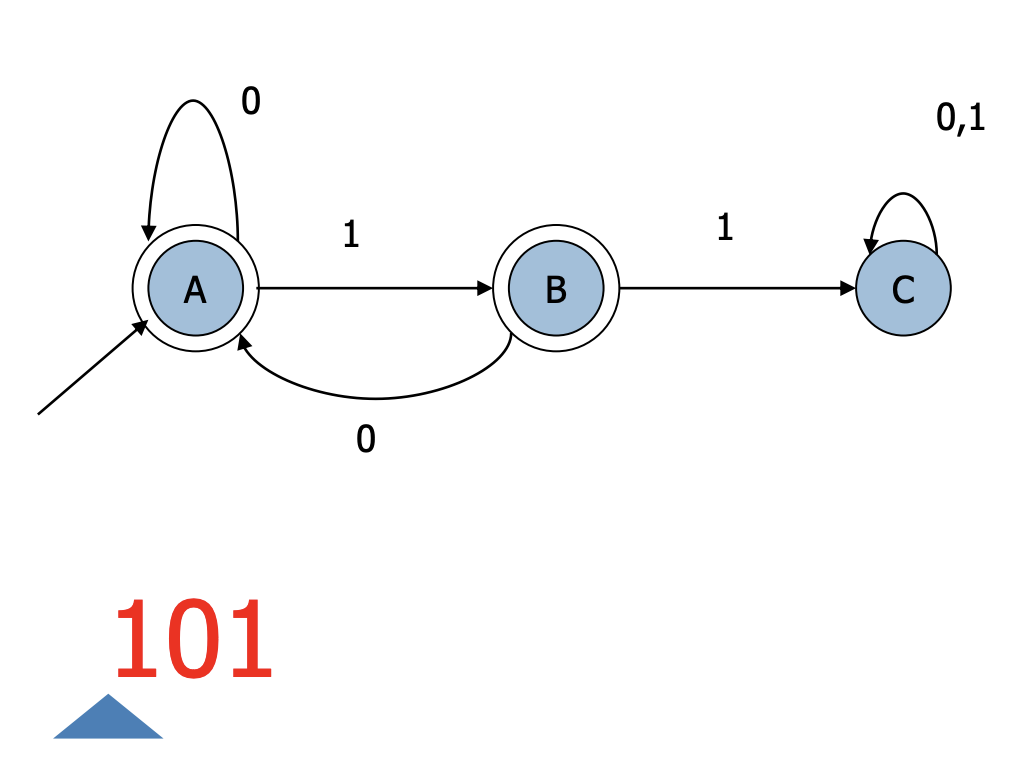
\includegraphics[width=0.5\textwidth]{img/afd/afd-1}\label{fig:figure}
    \end{figure}

    \begin{figure}[H]
        \centering
        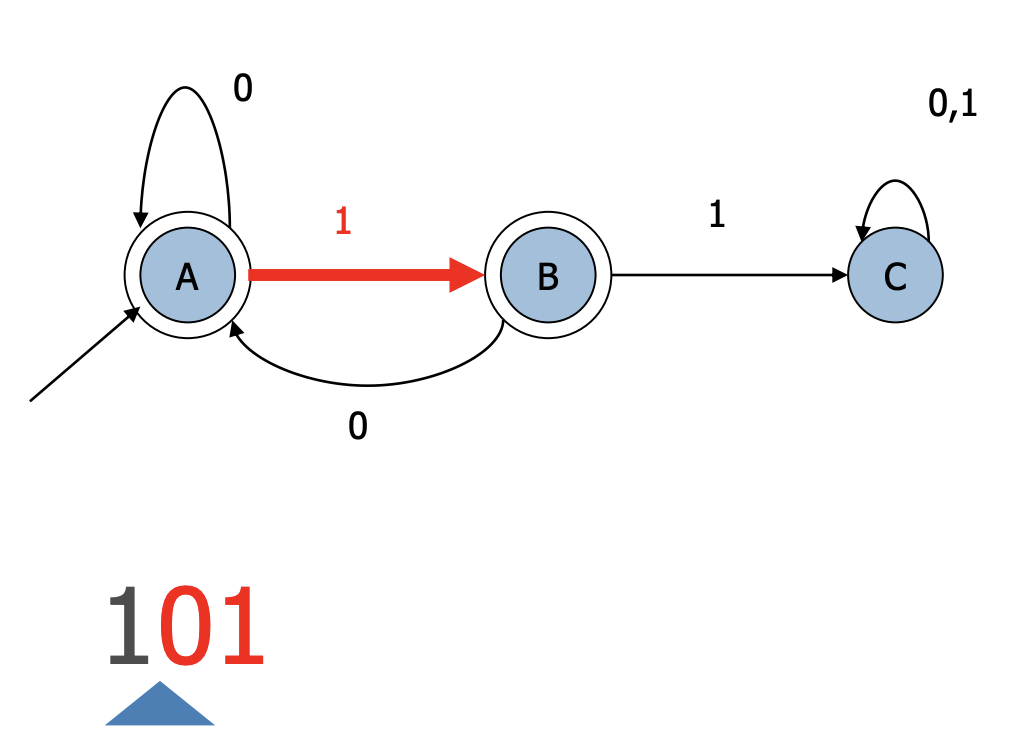
\includegraphics[width=0.5\textwidth]{img/afd/afd-2}\label{fig:figure2}
    \end{figure}

    \begin{figure}[H]
        \centering
        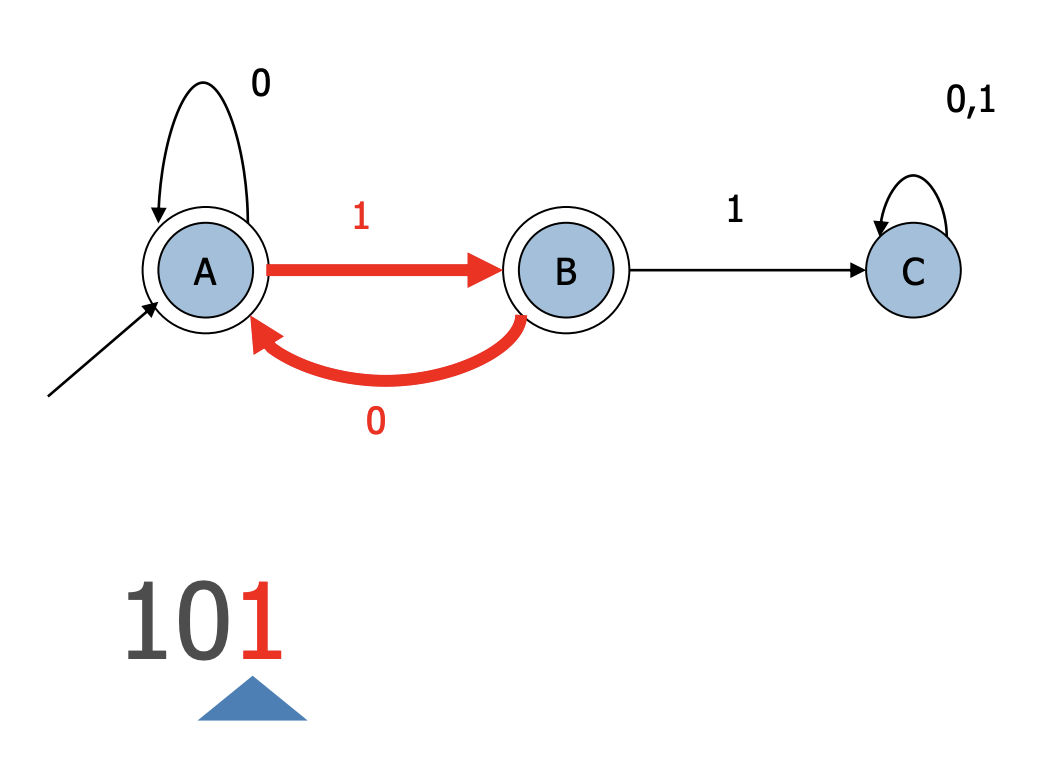
\includegraphics[width=0.5\textwidth]{img/afd/afd-3}\label{fig:figure3}
    \end{figure}

    \begin{figure}[H]
        \centering
        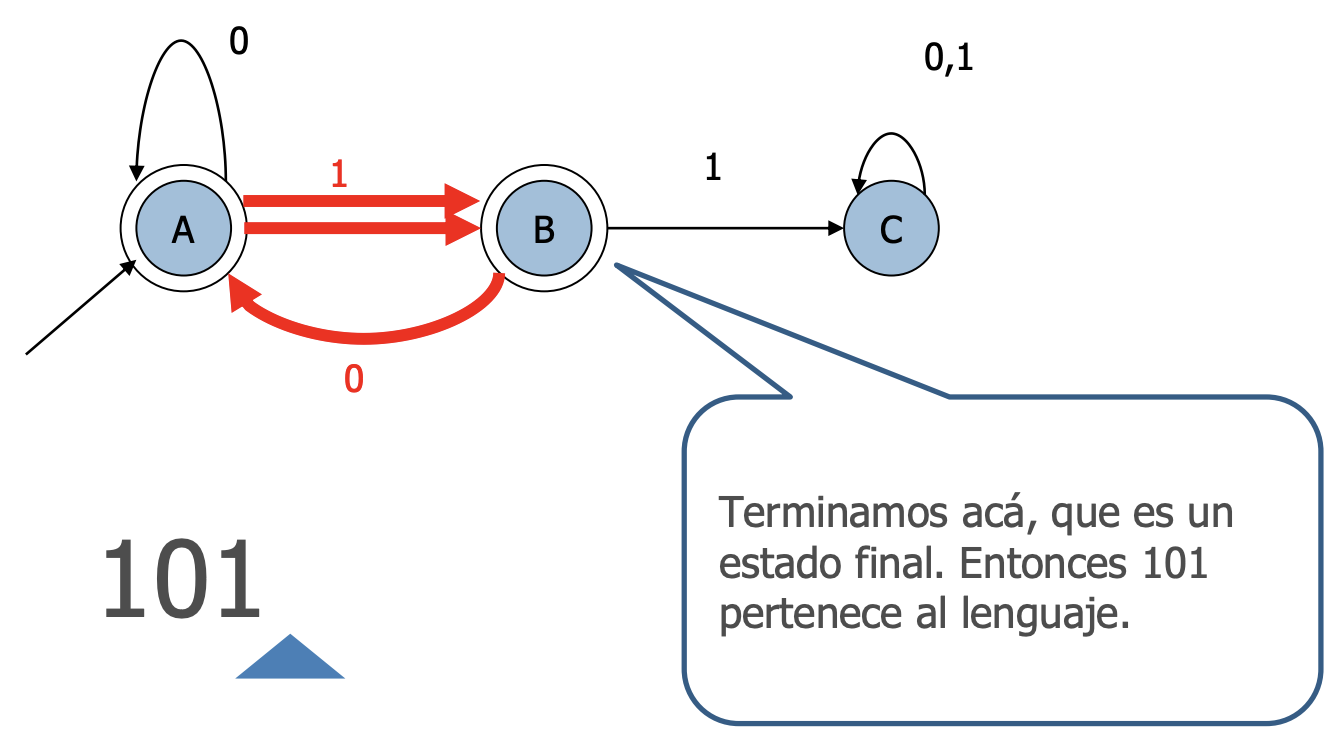
\includegraphics[width=\textwidth]{img/afd/afd-4}\label{fig:figure4}
    \end{figure}

    Luego, el lenguaje de nuestro AFD es: $\{w | w \in \{0,1\}^{\ast} \text{ y } w \text{ no tiene dos 1s consecutivos}\}$

    \subsection{Definición Formal de AFD}\label{subsec:definicion-formal-de-afd}

    Formalmente, un AFD es un formalismo para definir lenguajes que consiste en:

    \begin{itemize}
        \item Un conjunto finito de estados $Q$.
        \item Un alfabeto de entrada $\Sigma$.
        \item Una función de transición $\delta$.
        \item Un estado inicial $q_0 \in Q$.
        \item Un conjunto de estados finales $F \subseteq Q$.
    \end{itemize}

    \subsubsection{Función de Transición}

    La función de transición tiene dos parámetros: un estado $q$ y un símbolo de entrada $a$, y devuelve el estado al que se mueve el AFD cuando está en el estado $q$ y recibe el input $a$. Esta función debe estar definida para todo par $(q, a)$, donde $q \in Q$ y $a \in \Sigma$. La notación que se utiliza para representar la función de transición es $\delta(q, a)$.

    \subsection{Representación Gráfica de un AFD}

    Un AFD puede ser representado como un grafo decorado, donde:

    \begin{itemize}
        \item Los estados son representados como vértices.
        \item Las aristas representan la función de transición.
        \item Una flecha sin etiqueta (o con la etiqueta 'Start') apunta al estado inicial.
        \item Los estados finales se indican con círculos dobles.
    \end{itemize}

    Esta representación gráfica proporciona una forma visual e intuitiva de entender cómo funciona un AFD.

    \subsection{Representación alternativa: Tabla de transición}

    Una forma alternativa de representar un AFD es mediante una tabla de transición. En esta tabla:

    \begin{itemize}
        \item Usamos una flecha (->) para indicar el estado inicial.
        \item Las columnas representan los símbolos de entrada.
        \item Las filas representan los estados.
        \item Un asterisco (*) antes de un estado indica que es un estado final.
    \end{itemize}

    A continuación se encuentra un ejemplo de cómo se vería una tabla de transición:

    \begin{figure}
        \centering
        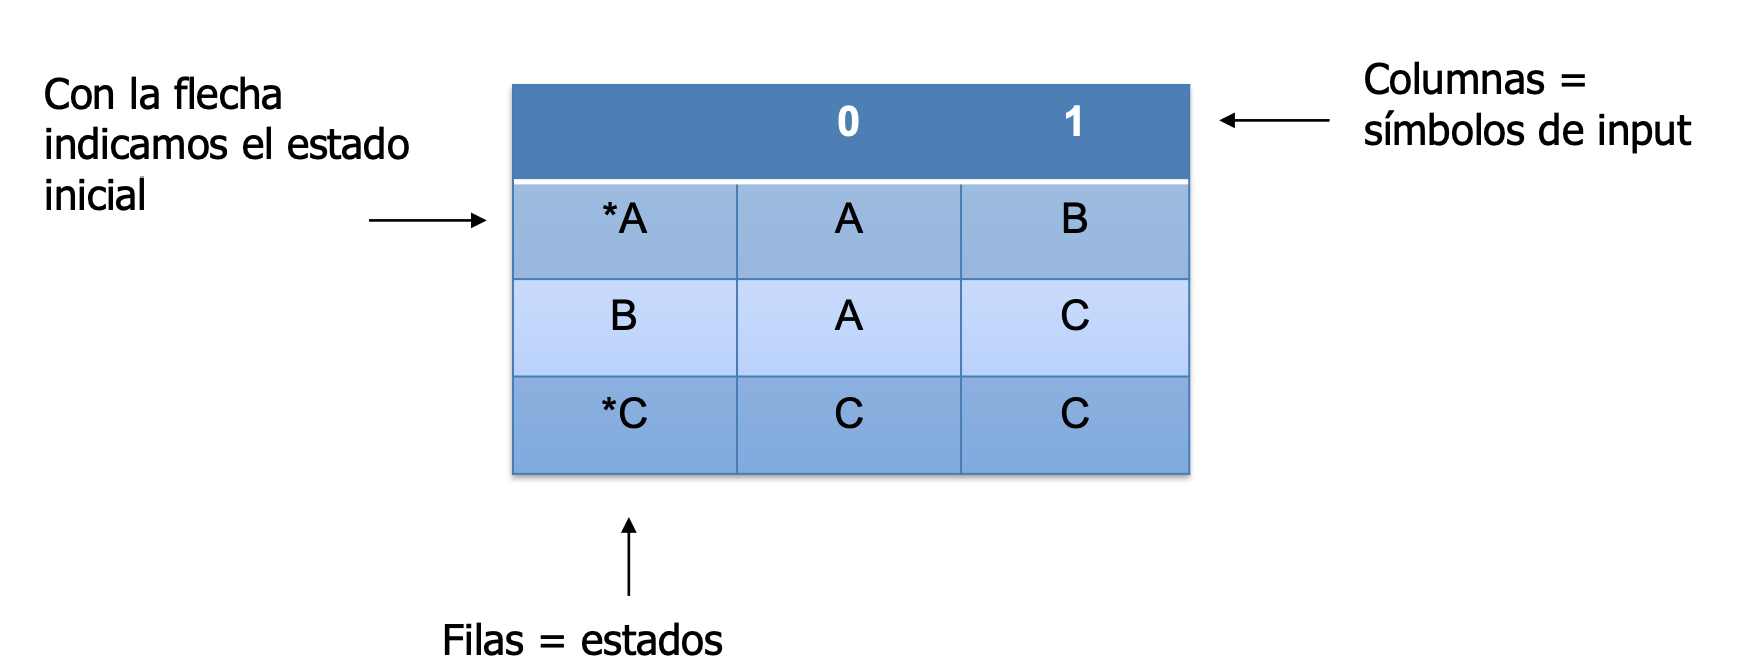
\includegraphics[width=\textwidth]{img/afd/afd-5}\label{fig:figure5}
    \end{figure}

    En esta tabla, el estado inicial es A, que también es un estado final. El estado C es otro estado final. La tabla muestra a qué estado se mueve el AFD para cada combinación de estado actual y símbolo de entrada.

    \subsection{Función de transición extendida}

    La función de transición extendida describe el efecto de un string de input sobre un AFD extendiendo la definición de $\delta$ para que tome un estado y un string. La definimos inductivamente de la siguiente manera:

    \subsubsection{Caso Base}

    $\delta(q, \epsilon) = q$

    \subsubsection{Caso Inductivo}

    $\delta(q, wa) = \delta(\delta(q, w), a)$, donde $w$ es un string y $a$ es un símbolo de input.

    \paragraph{Convención}

    $w, x, y, z$ son strings.

    $a, b, c, \ldots$ son caracteres sueltos.

    La $\delta$ extendida se computa para un estado $q$ e inputs $a_1a_2 \ldots a_n$ siguiendo un camino en el grafo de transiciones, comenzando en $q$ y seleccionando secuencialmente las aristas con etiquetas $a_1, a_2, \ldots, a_n$.

    \subsection{El lenguaje de un AFD}

    Los autómatas de todas clases definen lenguajes. Si $A$ es un autómata, $L(A)$ es su lenguaje. Para un AFD $A$, $L(A)$ es el conjunto de strings que llevan del estado inicial a uno de los estados finales.

    Formalmente: $L(A) = \{w | \delta(q_0, w) \in F\}$.

    \subsection{Más ejemplos}

    A continuación, se presentan más ejemplos de Autómatas Finitos Determinísticos (AFD):

    \subsubsection{AFD que reconozca todos los strings binarios que comiencen con 00}

    \begin{figure}[H]
        \centering
        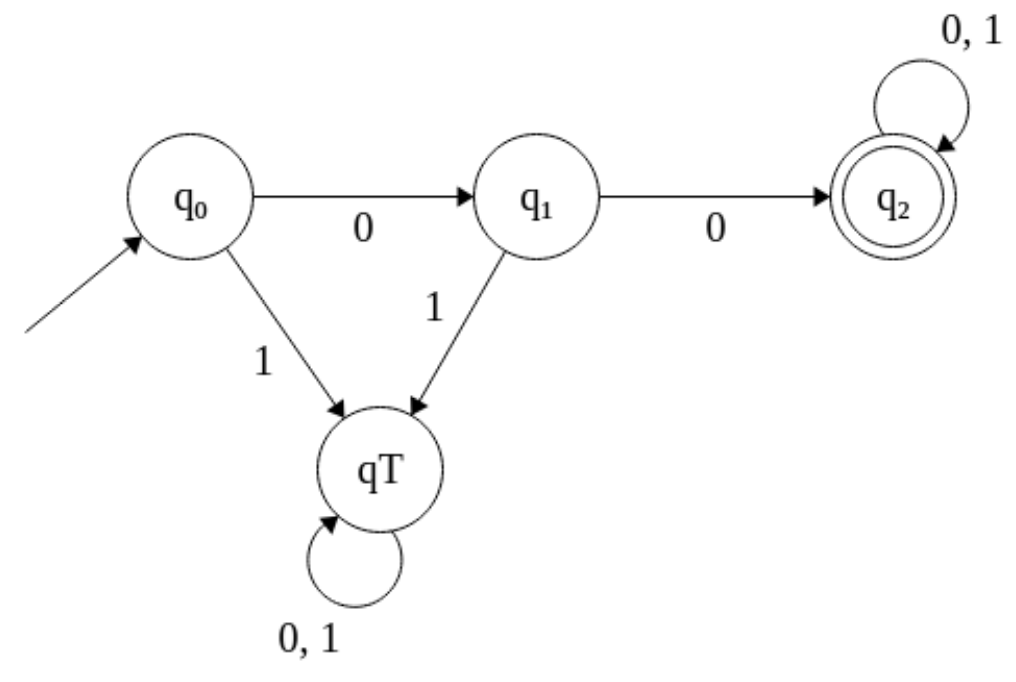
\includegraphics[width=\textwidth]{img/afd/afd-6}\label{fig:figure6}
    \end{figure}

    \subsubsection{AFD que reconozca todos los strings binarios que no comiencen con 00}

    \begin{figure}[H]
        \centering
        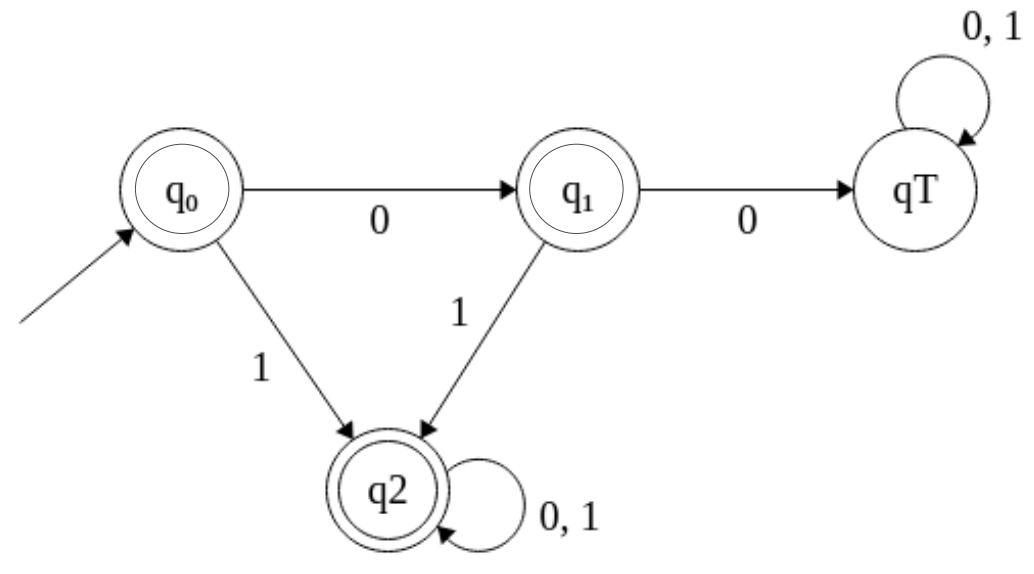
\includegraphics[width=\textwidth]{img/afd/afd-7}\label{fig:figure7}
    \end{figure}

    \subsubsection{AFD que reconozca todos los strings binarios que contengan al menos un 0}

    \begin{figure}[H]
        \centering
        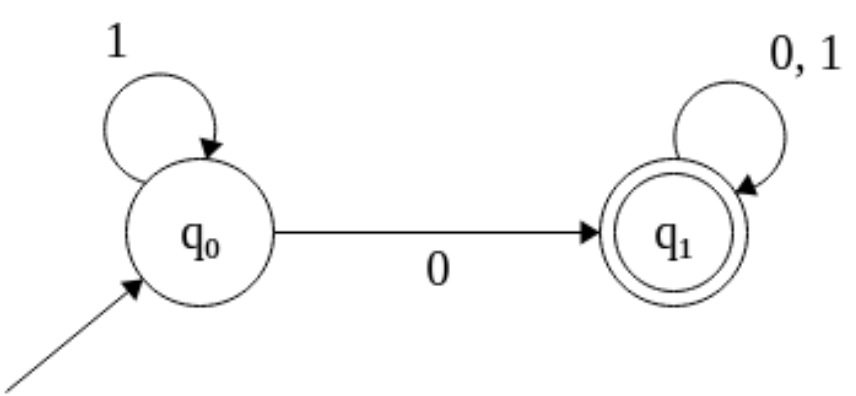
\includegraphics[width=\textwidth]{img/afd/afd-8}\label{fig:figure8}
    \end{figure}

    \subsubsection{AFD que reconozca todos los strings binarios tales que la cantidad de 1s sea par}

    \begin{figure}[H]
        \centering
        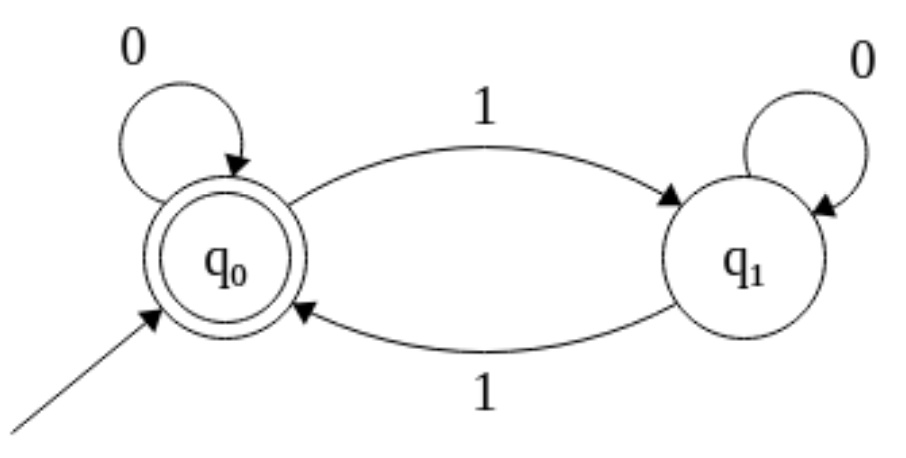
\includegraphics[width=\textwidth]{img/afd/afd-9}\label{fig:figure9}
    \end{figure}

    \newpage


    \section{Lenguajes Regulares}

    Un lenguaje $L$ se considera regular si puede ser reconocido por un Autómata Finito Determinista (AFD). El AFD debería aceptar únicamente cadenas de $L$, rechazando todas las demás. Algunos lenguajes no son regulares. Los lenguajes regulares pueden ser descritos de varias maneras, como mediante expresiones regulares. Aparecen en diferentes contextos y poseen propiedades útiles, por ejemplo, para representar números de punto flotante.

    \subsection{Ejemplos de lenguajes regulares y no regulares}

    Consideremos el lenguaje regular $L_3 = \{ w | w \in \{0,1\}^* \text{ tal que } w \text{ tiene un número par de 1s y un número par de 0s}\}$. Este lenguaje es regular porque puede ser reconocido por un Autómata Finito Determinístico (AFD).

    \begin{figure}[H]
        \centering
        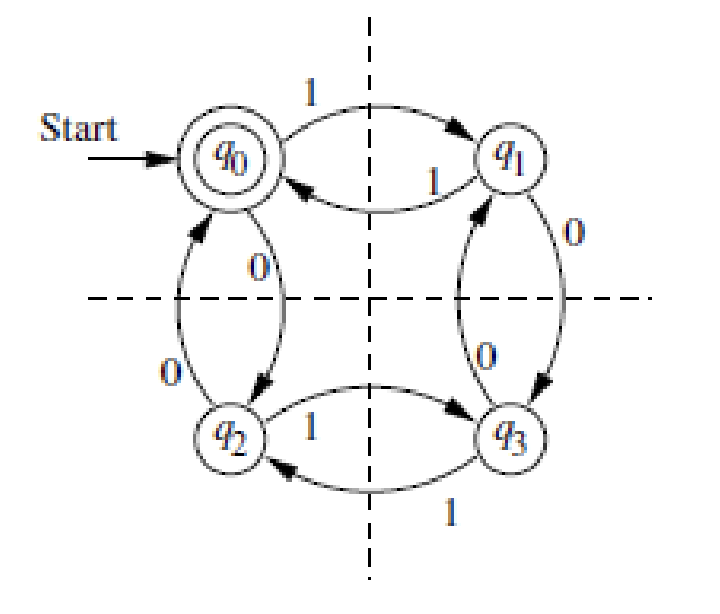
\includegraphics[width=0.5\textwidth]{img/afd/afd-10}\label{fig:figure10}
    \end{figure}

    Ahora consideremos el lenguaje $L_1 = \{0^n1^n | n \geq 1\}$. Este lenguaje no es regular porque no puede ser reconocido por un AFD. En este lenguaje, el número de 0s y 1s debe ser igual, lo cual no puede ser determinado por un AFD.

    Consideremos el lenguaje $L_2 = \{1, 0110, 00111100, 00011111111000, 000011111111111111110000, \ldots\}$. Este lenguaje es una secuencia de cadenas donde cada cadena tiene un número de 1s que es una potencia de 2. Este lenguaje también es no regular.

    Finalmente, consideremos el lenguaje que contiene cadenas con 16 1s. Este lenguaje es regular porque puede ser reconocido por un AFD que acepta cadenas con exactamente 16 1s.


    \section{Lema de Pumping}

    El lema de pumping se utiliza para reconocer un lenguaje no regular (los AFDs modelan solo lenguajes regulares). De manera intuitiva, si $L$ es regular, existe un número $n$ tal que las cadenas en $L$ con longitud mayor a $n$ pueden descomponerse en tres partes, y esas tres partes pueden repetirse infinitamente manteniendo la cadena resultante en $L$.

    \subsection{Analogía con el Principio del Palomar}

    Las tres partes son: $X$ (inicio), $Y$ (medio) y $Z$ (final). Todos los lenguajes regulares tienen esta estructura. Si no la tienen, se puede demostrar que no son regulares. Todos los lenguajes regulares pueden ser modelados por algún AFD.

    \subsection{Formalmente}

    \textbf{Teorema (Lema de Pumping para Lenguajes Regulares):} Sea $L$ un lenguaje regular. Entonces existe una constante $n$ (dependiente de $L$) tal que para cada cadena $w$ en $L$ con $|w| \geq n$, podemos descomponer $w$ en tres cadenas $w = xyz$ tal que:

    1. $y \neq \epsilon$
    2. $|xy| \leq n$
    3. Para todo $k \geq 0$, la cadena $xy^kz$ está en $L$.

    \subsubsection{Recordatorio: El Principio del Palomar (Formal)}

    Dados dos números naturales $k$ y $m$, si se distribuyen $n = km + 1$ objetos en $m$ conjuntos, al menos uno de los conjuntos contendrá (al menos) $k + 1$ elementos.

    \subsubsection{Suposiciones}

    Supongamos que $L$ es regular, con $L = L(A)$ para un AFD $A$. Supongamos que $A = < Q, \Sigma, \delta, q_0, F>$ tiene $n$ estados. Sea $w = a_1a_2 \ldots a_m$, $m \geq n$ cualquier cadena. Ahora, para $r = 0, 1, \ldots, n$, definimos $p_r = q_0$ para $r = 0$ y $p_r = \delta(q_0, a_1 \ldots a_r)$ para $r > 0$.

    \subsubsection{Aplicación del Principio del Palomar}

    Por el Principio del Palomar, no es posible que los $n + 1$ $p_r$s sean todos distintos. Así que tomemos dos enteros $i$ y $j$, con $0 \leq i < j \leq n$, tal que $p_i = p_j$.

    \subsubsection{Descomposición de $w$}

    Ahora podemos descomponer $w = xyz$ de la siguiente manera: $x = a_1a_2 \ldots a_i$, $y = a_{i+1}a_{i+2} \ldots a_j$, $z = a_{j+1}a_{j+2} \ldots a_m$. Observación: $y \neq \epsilon$, Observación: $|xy| \leq n$.

    \begin{figure}[H]
        \centering
        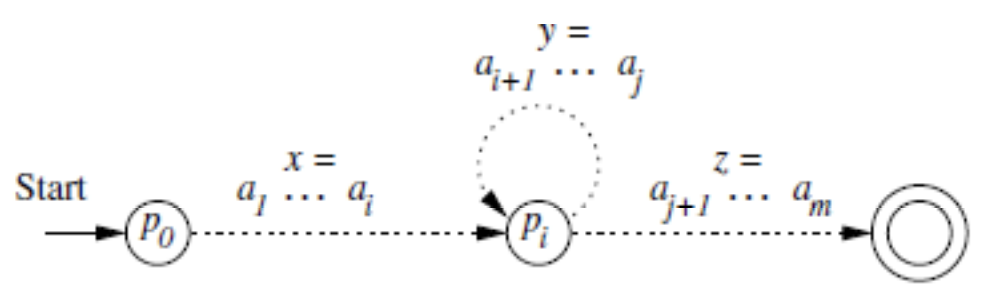
\includegraphics[width=0.5\textwidth]{img/afd/afd-11}\label{fig:figure11}
    \end{figure}

    \subsubsection{¿Qué sucede cuando $A$ recibe $xy^kz$ como entrada, para $k \geq 0$?}

    Si $k = 0$, $A$ acepta $xz$. Si $k > 0$, $A$ acepta $x(y^k)z$.


    \newpage


    \section{Autómatas Finitos No Determinísticos (AFND)}

    Los Autómatas Finitos No Determinísticos, también conocidos como AFND, son una extensión de los Autómatas Finitos Determinísticos (AFD) que permiten múltiples transiciones para un mismo símbolo de entrada y estado.

    \subsection{No determinismo}

    El concepto de no determinismo es fundamental para entender los AFND. Un autómata es no determinístico si, a partir de un estado dado, existe más de una transición posible para un mismo símbolo de entrada.

    \subsubsection{Estados simultáneos}

    Un AFND tiene la capacidad de estar en varios estados simultáneamente. Esto significa que, a partir de un estado y un símbolo de entrada, el autómata puede transitar a varios estados a la vez.

    \subsubsection{Transiciones a conjuntos de estados}

    En un AFND, las transiciones desde un estado con un símbolo de entrada pueden ser a un conjunto de estados. Esto contrasta con los AFD, donde cada par de estado y símbolo de entrada determina un único estado siguiente.

    \subsubsection{Aceptación de cadenas}

    Un AFND comienza su ejecución en un estado inicial. Acepta una cadena de entrada si existe alguna secuencia de transiciones que, partiendo del estado inicial y siguiendo los símbolos de la cadena de entrada, lleva a un estado final.

    \subsubsection{Intuición sobre el no determinismo}

    Intuitivamente, se puede pensar que un AFND siempre \("\)adivina correctamente\("\) el camino a seguir cuando se encuentra con varias transiciones posibles para un mismo símbolo de entrada. Si existe al menos un camino que lleva a un estado final, el AFND aceptará la cadena de entrada.\\\\
    Imagina que estás en un laberinto y llegas a un punto donde hay varios caminos posibles a seguir. En un escenario determinístico, solo podrías seguir un camino y tendrías que vivir con las consecuencias de esa elección. Sin embargo, en un escenario no determinístico, como el que maneja un AFND, podrías explorar todos los caminos simultáneamente. Si al menos uno de esos caminos te lleva a la salida del laberinto, entonces has "adivinado correctamente" y has encontrado una solución.

    \subsection{Descripción formal de un AFND}

    Un Autómata Finito No Determinístico (AFND) se define formalmente como:

    \begin{itemize}
        \item Un conjunto finito de estados $Q$.
        \item Un alfabeto de entrada $\Sigma$.
        \item Una función de transición $\delta$.
        \item Un estado inicial $q_0 \in Q$.
        \item Un conjunto de estados finales $F \subseteq Q$.
    \end{itemize}

    \subsubsection{Función de transición de un AFND}

    La función de transición $\delta(q, a)$ de un AFND es una función $\delta : Q \times \Sigma \rightarrow P(Q)$ cuya imagen es un conjunto de estados. Esta función se extiende a cadenas de la siguiente manera:

    \begin{itemize}
        \item Caso base: $\delta(q, \epsilon) = \{q\}$.
        \item Caso inductivo: $\delta(q, wa) = \bigcup_{p \in \delta(q, w)} \delta(p, a)$.
    \end{itemize}

    Intuitivamente, la función de transición extendida $\delta(q, wa)$ en un Autómata Finito No Determinístico (AFND) se puede describir como la unión sobre todos los estados $\delta(p, a)$, con $p \in \delta(q, w)$

    \begin{tikzpicture}[->,>=stealth',shorten >=1pt,auto,node distance=3cm,
        semithick]
        \tikzstyle{every state}=[fill=red,draw=none,text=white]

        \node[state] (A)                    {$\sigma(q, a)$};
        \node[state] (B) [above right of=A] {$q_1$};
        \node[state] (C) [below right of=A] {$q_n$};
        \node[state] (D) [right of=A]       {$q_2$};
        \node[state] (E) [right of=B]       {$\sigma(q_1, w)$};
        \node[state] (F) [right of=C]       {$\sigma(q_n, w)$};
        \node[state] (G) [right of=D]       {$\sigma(q_2, w)$};
        \node[state] (H) [right of=E]       {$q_{11} \ldots q_{1n}$};
        \node[state] (I) [right of=F]       {$q_{n1} \ldots q_{nn}$};
        \node[state] (J) [right of=G]       {$q_{21} \ldots q_{2n}$};

        \path (A) edge node {} (B)
        edge node {} (C)
        edge node {} (D)
        (B) edge node {} (E)
        (C) edge node {} (F)
        (D) edge node {} (G)
        (E) edge node {} (H)
        (F) edge node {} (I)
        (G) edge node {} (J);
    \end{tikzpicture}

    Luego, la unión de los estados es igual a

    \[
        \sigma(q, wa) = \{q_{11}, \ldots, q_{1n}, q_{21},\ldots, q_{2n}, q_{n1},\ldots, q_{nn}\}
    \]

    \subsubsection{Lenguaje de un AFND}

    Un string es aceptado por un AFND si $\delta(q_0, w)$ contiene al menos un estado final, es decir que habiendo consumido todos los caracteres de un string, en alguno de los \("\)caminos\("\) del AFD se llega a un estado final. El lenguaje de un AFND es el conjunto de strings que acepta.

    \subsection{Ejemplos}

    \subsubsection{AFND que reconozca todos los strings binarios que comiencen con 00}

    A continuación, se presenta un ejemplo de un Autómata Finito No Determinístico (AFND) que reconoce si el string binario comienza con 00.

    \begin{figure}[H]
        \centering
        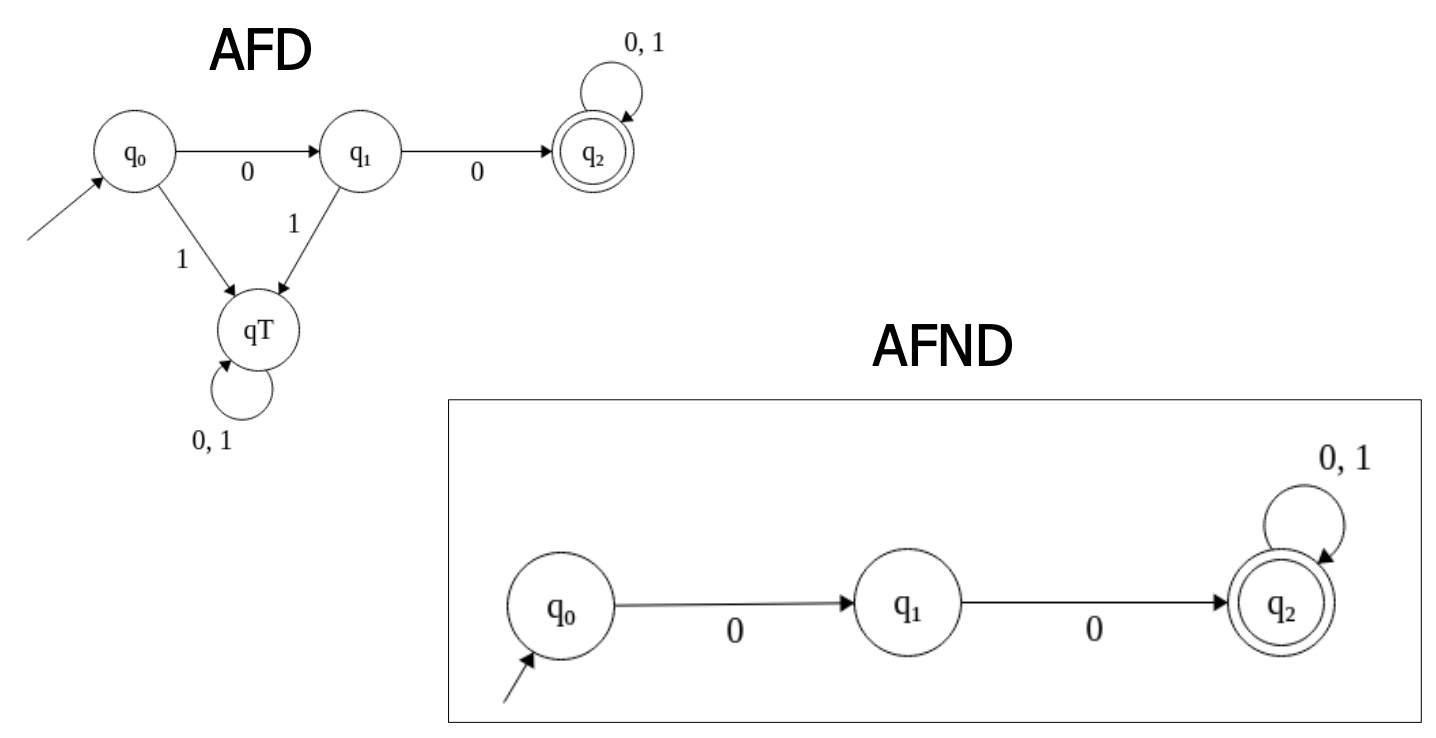
\includegraphics[width=\textwidth]{img/afnd/afnd-1}\label{fig:figure12}
    \end{figure}

    \subsubsection{AFND que reconozca todos los strings del alfabeto \{a, b, c\} que contengan al menos 2 ocurrencias del mismo caracter}

    A continuación, se presenta un ejemplo de un Autómata Finito No Determinístico (AFND) que reconoce si el string del alfabeto \{a, b, c\} contiene al menos 2 ocurrencias del mismo caracter.

    \begin{figure}[H]
        \centering
        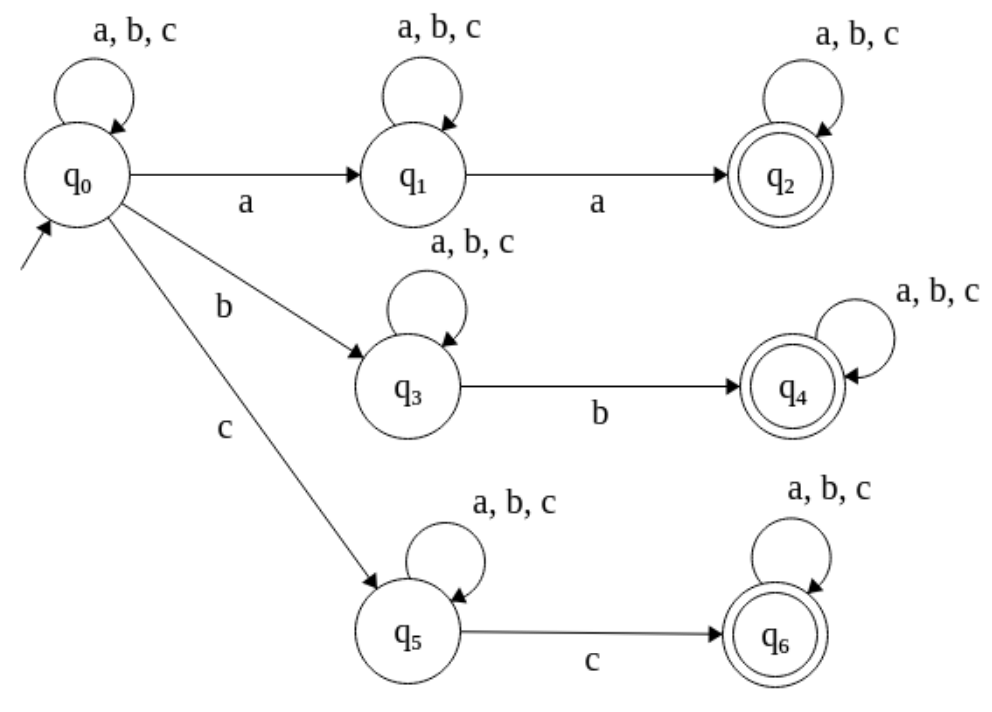
\includegraphics[width=\textwidth]{img/afnd/afnd-2}\label{fig:figure13}
    \end{figure}


\end{document}